% Chapter 2

\chapter{Background} % Main chapter title

\label{Chapter2} % For referencing the chapter elsewhere, use \ref{Chapter2} 

\lhead{Chapter 2. \emph{Background}} % This is for the header on each page - perhaps a shortened title

%----------------------------------------------------------------------------------------

In this chapter we present a detailed background survey of different techniques for segmenting single neurons from confocal microscopy. As we have mentioned earlier, we restrict ourselves to the case of detecting single neurons, and therefore techniques which fall under the multi neuron category, or are based on other imaging modalities (such as EM, two photon microscopy) are excluded from the discussion. 

The different neuronal components (also popularly known as neuronal processes in biology) such as dendrites and axons, imaged via confocal microscope typically exhibit filamentous appearance. A majority of the neuron image analysis algorithms exploit the filamentous nature of the structures to devise tracing methodologies in presence of background noise and clutter. Vascular or filamentous/tubular structures occur in abundance in medical imaging. This includes, but are not restricted to, retinal blood vessels, blood vessels and arteries in the brain and other organs imaged via CTA, human arteries as seen in ultrasound images etc. A majority of these images suffer from poor contrast and background noise and thereby require a preprocessing step to enhance the vascular structures before performing segmentation. 

Perhaps one of the most widely used and well known vessel enhancing method was proposed by Frangi \textit{et al} \cite{frangi_vesselness}. In the recent years, there have been significant research to develop robust algorithms to improve vessel detection from low contrast imagery. This includes 3D line filters due to Sato \textit{et al}.\cite{sato1998three}, diffusion based methods\cite{manniesing2006vessel} and steerable ridge detectors \cite{jacob2004steerable}. Vessel enhancement is an integral step in many tracing and segmentation algorithms, and will be discussed in significant detail in the next few chapters of this dissertation.


\section{Neuron segmentation and tracing}

The terms tracing and segmentation are often used interchangeably in the relevant literature. In most cases, tracing refers to the algorithms that focus on reconstruction of the neuron by identifying the centerline of the filaments. Segmentation algorithms, on the other hand are more traditional and aim at delineating the entire neuronal structure using traditional segmentation tools such as thresholding, morphological operations, connected component analysis, active contours, graph cuts etc \cite{bovik2010handbook}. The neuron tracing can be obtained from the segmented result by computing the centerline of the binary segments using skeletonization algorithms \cite{bovik2010handbook}.  However, before we discuss the algorithms for neuron tracing, let us briefly talk about the biological motivation and imaging technique for data acquisition.

\subsection{Challenges in image processing}

Confocal microscopy is a popular method for imaging single neuron cells. The ability to visualize neurons at a single cell resolution is a significant step towards automated structure identification.  Confocal laser scanning microscopes (CLSM) use focused laser beams to excite selectively tagged neurons (which are labeled with a florescent protein) to emit energy in form of photons, which are subsequently absorbed by a photodetector to create an image of the objects at the particular optical plane. Out of plane scatter is suppressed by the detector aperture, thus allowing sharper image formation.  Information can be collected  from different focal planes by altering the focal length of the system, thus creating multiple slices (z-stacks), which are eventually fused to form a 3D image of the specimen. 


Like many other light microscopy techniques, neuron imaging using confocal microscopy comes with its own set of challenges. First, most images are low contrast and suffer from low signal to noise ratio. Photobleaching effect restricts the imaging time, which directly affects the signal intensity and contrast. Also, irregular photon emission from the filaments, especially those at greater depths, creates inhomogeneous signal intensity and renders a fragmented appearance of the neurites. Finally, the images are affected by photon noise and clutter resulting from non neuronal fluorescing tissues. All these aspects make image processing challenging and a suitable neuron tracer needs to manage these artifacts using sophisticated image processing.  Fig.~\ref{fig:neuron_stack_demo} shows an example of the imaging artifacts discussed here.
\begin{figure}[t]
\centering
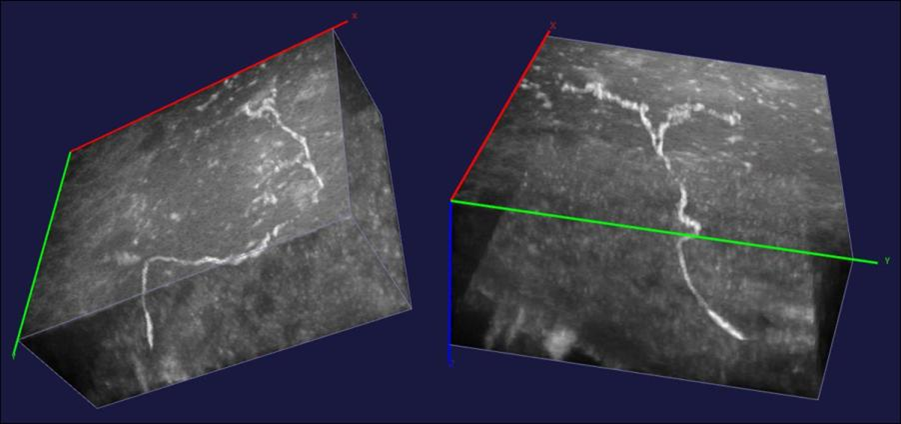
\includegraphics[width=0.8\textwidth]{images/3D_demo}	
\caption[Imaging artifacts]{A 3D confocal microscopy image of Drosophila interneuron is shown from two viewing angles. The image is degraded by low contrast and inhomogeneous illumination of the neurite. Furthermore, presence of noise and background clutter deteriorates the image quality.}
\label{fig:neuron_stack_demo}
\end{figure}

\subsection{Neuron tracing strategies}
In this section we are going to highlight some popular neuron tracing and segmentation works. Most of these tools are extensively used by biologists for segmentation of single neurons. However, the list is  definitely not exhaustive and more algorithms are being developed each day as the field continues to grow.

We can broadly categorize the neuron segmentation schemes in two basic approaches. The first set of methods use user defined (or automatically detected) initial seed points to perform tracing in a local exploratory manner. Such methods are popularly known as \textit{tracing} algorithms or \textit{tracers}, since the algorithms locally trace the neuron centerlines. The second category of algorithms avoid seed initialization and perform segmentation using a combination of local and global features. In the next few subsections, we will discuss a few popular neuron tracing and segmentation algorithms. 

\subsubsection{NeuronJ}
One of the earlier works in neuron tracing was proposed by Meijering \textit{et al.}\cite{meijering2004design}. The tracing algorithm, NeuronJ, is a 2D neuron tracer, which uses specialized steerable ridge detector kernels \cite{jacob2004steerable} to determine the evidence of a neuron filament, which the authors call \textit{neuriteness}. A semi automated graph based tracing method \textit{Livewire} \cite{livewire} is then used to trace the neurite centerline, using evidence of neuriteness from the ridge detector response. 

NeuronJ is widely used in the scientific community for 2D tracing, and it owes its popularity to its robustness and simplicity, and is available as a plugin for the open source, bio-imaging software ImageJ\cite{imageJ}. However, the method is custom made for 2D imagery only, and carrying out such user interactive tracing in 3D appears less trivial. Also, the algorithm relies significantly on user assistance, especially for determining branch points and neurite terminals. As a result, the applicability of this tool is somewhat limited for high throughput analysis.
 
\subsubsection{Simple Neurite Tracer}
Simple Neurite Tracer\cite{SNT} is another open source, publicly available, semi-automated 3D neuron tracer.
Simple Neurite Tracer (SNT) falls under the category of seed-based tracing algorithm, where the user selects a set of initial points on the neuron centerline. A graph is then created, with these seed points serving as the nodes of the graph, and the edge weights depending on their relative distance and the vessel intensity at the seed locations. A shortest path algorithm\cite{dijkstra1959note} is then deployed to compute the best possible path between the adjacent seeds. 

Like many vessel tracing algorithms, SNT also uses vessel enhancement technique \cite{frangi_vesselness,sato1998three} for determining the shortest path between the seeds. Similar to NeuronJ, SNT is also available as a plugin for ImageJ. However, the major drawback of SNT include the excessive use of human assistance (for seed detection, merge point identification etc.) for tracing. That being said, SNT is popular among biologists and is often used as a post processing platform for correcting or editing neuron reconstructions from automated tracers.

\subsubsection{Vaa3D and associated algorithms}
Vaa3D\cite{peng_v3d} is a neuron tracing software suit which is gaining significant popularity in the recent years. The C++ based tracing suit hosts a number of neuron tracing algorithms, both seed based and automated. One popular method, Graph Augmented Deformable model (GD model) was proposed by Peng \textit{et al}\cite{peng_GAD}. The GD model performs neuron tracing based on some user chosen seeds, which are typically chosen as the neurite terminals. With these set of chosen locations, tracing is performed between the pairwise seeds using a deformable, shortest path approach. Fast and accurate segmentation is possible using the above mentioned approaches if the neuron morphology is simple and the image noise level is low. Recent algorithms proposed by the same group \cite{peng_anisotropicPS,peng_APP} attempts to make the tracing more user independent by initially performing an over segmentation by choosing a conservative threshold, followed by pruning to delete unwanted components. 

\subsubsection{k-Minimum Spanning Tree}
Gonzalez \textit{et al}. \cite{turetken_Diadem} introduced a graph theoretic technique to delineate the optimal neuronal tree from an initial set of seeds by computing a k-Minimum Spanning Tree. To automatically generate the seed points, the authors propose using a supervised learning methodology to determine potential neurite locations. This neuron probability map is importance sampled to generate a set of seeds, with special care taken to preserve the important locations such as tips and bifurcations. 

Since the minimum spanning tree of a graph created from all the nodes can contain non neuronal clutter, the authors propose a novel solution by posing am optimization problem that finds the k\textsuperscript{th} minimum spanning tree. An approximate solution to this NP-hard problem is realized by minimizing a global energy function in a linear integer programming framework. Recently, there have been efforts to improve the accuracy of the algorithm, by using a different optimization criteria\cite{turetken_MIP}. 

\subsubsection{NeuronStudio}
NeuronStudio\cite{wearne_neuronStudio} is a neuron segmentation software toolkit. Unlike the aforementioned methods, which are essentiially tracing techniques and rely on initial seed selection, NeuronStudio is an example of a traditional segmentation algorithm. The algorithm implemented is known as \textit{voxel scooping} method\cite{rodriguez_voxelscoop}. It assumes that the neurites are locally tubular filaments and iteratively searches for voxel clusters in a manner similar to region growing. A pruning step is then deployed to eliminate spurious end nodes.

The biggest aspect of NeuronStudio is that it is relatively less dependent on user interaction, and segmentation only requires a single seed location to identify the starting position for region growing. However, the region growing algorithm becomes less stable when the images are degraded by low contrast, and region leakage becomes an issue for processing.

\subsubsection{Open-Curve Snake}
The Open-Curve Snake method\cite{wang_Roysam_open_curve,cai_ISBI} is implemented using open ended parametric active contours. This can be considered to be a tracing method, where the 1D curves are evolved along the vessel centerline to perform tracing. An external force field is suitably designed for curve evolution, which encourages the trace to lie along the neuron centerline. A preprocessing step based on tensor voting \cite{roysam_tensorvoting} is also used to enhance the neuron contrast and the snake initialization is performed by using graph cuts\cite{graph_cut} to get an initial overestimate of the neurite locations. Combined with a post-processing step to eliminate false filaments, this method is efficient in segmenting neuronal structures from low SNR confocal stacks. However, due to the inability of parametric active contours to naturally handle topological changes such as object merging, neurite branch point detection depends requires a non-trivial post processing to determine snake merging at the junctions.
 
\subsubsection{Tree2Tree}
Tree2Tree \cite{basu_T2T_journal} aims to solve the neuron segmentation problem in a graph theoretic framework. Unlike traditional seed selection approaches, where manually designated points are treated as the nodes of the graph, an initial segmentation algorithm is devised to produce a set of disjoint binary connected components. Connectivity between the components is analyzed based on their separating distance and orientation, which determines the weights of the graph edges to perform segmentation using a minimum spanning tree approach. 

Although the primary contribution of Tree2Tree is to connect the fragmented neurite segments automatically, this connectivity analysis relies on heavily on the initialization. Noise and clutter in the images create undesired artifacts in the global segmentation, resulting in loss of structural information. Moreover, linking the components based on their relative geometric orientation requires computation of the leaf-tangents from the object centerlines, which is sensitive to the irregularities of the neurite surface. One drawback of Tree2Tree is that the disjoint neighboring neurite fragments are connected by a splined curve, which may not coincide with the actual neurite location in the image. This aspect of Tree2Tree is addressed in Tree2Tree2\cite{mukherjee_T2T_2}, which will be discussed in more details in Chapter  \ref{T2T2_chapter}.

\subsubsection{Other methods}
Apart from the above mentioned algorithms which are popular in the scientific community since the implementation is readily available, there are many more tracing methodologies that deserve mention. Al-Kofahi \textit{et al}. \cite{al_kofahi} used the medial response of multiple directional templates to determine the  direction to generate successive seed points along the neuron medial axis. This local tracing method shows good performance in high-contrast images, but requires continuity in the neuron branches for reliable segmentation. Other notable neuron tracers include the wavelet based algorithm due to \cite{dima_wavalet}, morphology and graph theory based technique of Chothani\textit{et al.} \cite{chothani2011automated} etc. 

Other methods of segmentation include the use of probabilistic region merging\cite{srinivasan2007automated},  tracking based algorithms \cite{wang2007dynamic,choromanska2012automatic} and active contours \cite{wang2011novel}. A survey of recent tools for neuron reconstruction is available due to Dr. Erik Meijering\cite{meijering_survey}.

The medical imaging community has performed substantial research in developing algorithms to detect and segment filamentous shapes in non-microscopy medical images \cite{lesage2009review}. While not related directly to neuron tracing or segmentation, methods for segmenting vasculature have been extended or modified for tracing neurons, and thereby deserve mention.

The CURVES algorithm by Lorigo \textit{et al}. \cite{lorigo2001curves} evolves a 1D curve along a 3D vessel centerline guided by the curvature of a 1D curve. Gooya \textit{et al}.\cite{gooya2008variational} developed an elegant and generalizable  regularization methodology to enhance the performance of the popular geometric curve evolution methods. The method allows for anisotropic curve propagation  which minimizes contour leakage when vessel edge information is weak. One apparent downside of this technique is that the ultimate solution somewhat depends on the shape of the initialized contour. Another recent work by Gooya \textit{et al}.\cite{gooya2012generalization} generalizes the flux maximizing flow \cite{flux_max} on Riemann manifolds and uses a vessel enhancing tensor, which improves segmentation when edge detection is less accurate.

Shang \textit{et al}. \cite{shang2011vascular} developed a vessel tracing algorithm where wider vessels are first segmented using a region based criteria. Then the eigenvectors of the hessian matrix are utilized to derive a geometric flow equation to segment the thinner vessels. Santamaria-Pang \textit{et al}. \cite{santamaria2007automatic} use a multistage procedure for detection of tubular structures in multi-photon imagery, which includes a pre-filtering stage to identify the filaments based on supervised learning. However, this requires offline learning of the model parameters and prior knowledge about the vessel appearance information, which necessitates a set of accurate training examples and demands extensive human involvement to generate the ground truth.

\section{Discussion}
The neuron segmentation algorithms discussed in this chapter are classified either as local tracers, or global segmentation techniques. We hypothesize that seed based local algorithms are useful if the imaged neurons are not too complicated structurally. In such scenarios, where manual seed selection is easy, reliable segmentation can be obtained. However, since automatically choosing the correct set of seed points is still an open problem, it is difficult to use the above mentioned techniques for high throughput, no intervention analysis. Also, since proper selection of seeds points is instrumental in these methods, the segmentation accuracy is sometimes compromised if a sub-optimal set of points is chosen. Furthermore, the connectivity analysis between the seeds assume uniform signal intensity, and noise and low contrast in the images may degrade the segmentation quality.

In contrast to the seed based local techniques, traditional segmentation approaches are more global, typically requiring an initial pre-processing of the image followed by a specialized segmentation step. Although a global approach may suffer from expensive computation, they are more suitable for neurite junction and end point detection.
Typically, such methods rely on a four stage processing pipeline -- enhancement, segmentation, centerline detection and post processing. However, despite being less dependent on user interaction, global segmentation algorithms should be adequately modeled to capture the finer details of neurite geometry, such as complex branching patterns, including twists and turns of filaments and should be capable of handling signal attenuation due to imaging artifacts.

Due to the aforementioned reasons, we refrain from using local seed based techniques for segmenting neurons. In the following chapters, three novel neuron segmentation methods are presented, which are completely automated and do not require manual identification of seed points for tracing. 